\documentclass[10pt,a4j]{jarticle}
%\usepackage{graphicx,wrapfig}
\usepackage{graphicx}
\setlength{\topmargin}{-1.5cm}
\setlength{\textwidth}{16.5cm}
\setlength{\textheight}{25.2cm}
\newlength{\minitwocolumn}
\setlength{\minitwocolumn}{0.5\textwidth}
\addtolength{\minitwocolumn}{-\columnsep}
%\addtolength{\baselineskip}{-0.1\baselineskip}
%
\def\Mmaru#1{{\ooalign{\hfil#1\/\hfil\crcr
\raise.167ex\hbox{\mathhexbox 20D}}}}
%
\begin{document}
\newcommand{\fat}[1]{\mbox{\boldmath $#1$}}
\newcommand{\D}{\partial}
\newcommand{\w}{\omega}
\newcommand{\ga}{\alpha}
\newcommand{\gb}{\beta}
\newcommand{\gx}{\xi}
\newcommand{\gz}{\zeta}
\newcommand{\vhat}[1]{\hat{\fat{#1}}}
\newcommand{\spc}{\vspace{0.7\baselineskip}}
\newcommand{\halfspc}{\vspace{0.3\baselineskip}}
\bibliographystyle{unsrt}
%\pagestyle{empty}
\newcommand{\twofig}[2]
 {
   \begin{figure}
     \begin{minipage}[t]{\minitwocolumn}
         \begin{center}   #1
         \end{center}
     \end{minipage}
         \hspace{\columnsep}
     \begin{minipage}[t]{\minitwocolumn}
         \begin{center} #2
         \end{center}
     \end{minipage}
   \end{figure}
 }
%%%%%%%%%%%%%%%%%%%%%%%%%%%%%%%%%
%\vspace*{\baselineskip}
\begin{center}
	{\Large \bf 2019年度 構造力学II 講義メモ1} \\
\end{center}
%%%%%%%%%%%%%%%%%%%%%%%%%%%%%%%%%%%%%%%%%%%%%%%%%%%%%%%%%%%%%%%%
\section{1次元軸力問題}
\subsection{強形式}
1次元軸力問題の支配方程式は
\begin{equation}
	\frac{d}{dx}\left(EA \frac{du}{dx}\right) + p =0, \ \ \left(x\in (0,l)\right)
	\label{eqn:gveq}
\end{equation}
で与えられる.ここで,
$u$は軸変位を,$E$はヤング率,$A$は部材の断面積を表し,$p(x)$は
部材軸方向に働く分布力で,単位長さあたりの力の次元を持つ.
式(\ref{eqn:gveq})は, 軸力$N$に関する釣り合い条件:
\begin{equation}
	\frac{dN}{dx}+p=0, \ \ \left(x\in (0,l)\right)
	\label{eqn:equiv_N}
\end{equation}
と,フックの法則:
\begin{equation}
	\sigma=E\varepsilon
	\label{eqn:Hooke}
\end{equation}
に由来するものである.なお,$\sigma$は軸方向の直応力を,
$\varepsilon$は直ひずみを表し,ひずみと変位の関係は
\begin{equation}
	\varepsilon = \frac{du}{dx},
	\label{eqn:dudx}
\end{equation}
軸力と応力の関係は
\begin{equation}
	\sigma=\frac{N}{A}
\end{equation}
である.
棒部材が図\ref{fig:fig1_1}のように支持されている場合,$x=0$と$x=l$における
境界条件(支持条件)は次のようになる.
\begin{eqnarray}
	u (0) &= & 0 
	\label{eqn:BC_u}
	\\
	N (l) &= & EA u'(l)=\bar F 
	\label{eqn:BC_N}
\end{eqnarray}
\begin{figure}[h]
	\begin{center}
	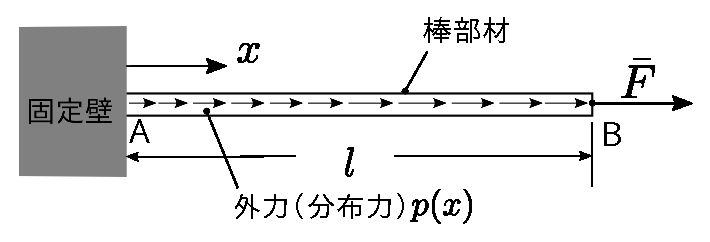
\includegraphics[width=0.4\linewidth]{fig1_1.eps} 
	\end{center}
	\caption{軸方向の外力$p(x)$と$\bar F$を受ける棒部材.} 
	\label{fig:fig1_1}
\end{figure}
以上のように,微分方程式と境界条件による問題の定式化を強形式(strong form)と呼ぶ.
\subsection{弱形式}
$\xi (x)$を$0\leq x \leq l$で定義された$\xi(0)=0$を満たす任意の関数であるとする.
$\xi (x)$を式(\ref{eqn:equiv_N})の両辺に掛け,$x=0$から$x=l$の範囲で次のように積分する.
\begin{equation}
	\int _0^l 
	\left(N'+p \right) \xi dx =0
	\label{eqn:int_gveq_xi}
\end{equation}
この式の左辺第一項を,部分積分を用いて変形すると,
\begin{eqnarray}
	\int _0^l N'\xi dx &= & \left[ N\xi \right]_0^l -\int_0^l N \xi'dx  
	\label{eqn:}
	\\
	&= & \bar F \xi(l)  -\int_0^l N \xi'dx  
\end{eqnarray}
となる.これを,式(\ref{eqn:int_gveq_xi})に代入すれば,次の関係が得られる.
\begin{equation}
	a(u,\xi)=b(\xi)
	\label{eqn:WF_N}
\end{equation}
ただし,$a(u,\xi)$と$b(\xi)$は以下の通りとする.
\begin{equation}
	a(u,\xi) = \int_0^l N \xi'dx  
	= \int_0^l EA u' \xi'dx  
	\label{eqn:blinf_N}
\end{equation}
\begin{equation}
	b(\xi)= \bar F \xi (l) + 
	\int_0^l p\xi dx 
	\label{eqn:linf_N}
\end{equation}
任意の$\xi(x)$(ただし$\xi(0)=0$)について式(\ref{eqn:WF_N})を満足する$u(x)$のうち,
$u(0)=0$となる$u(x)$("弱解"と呼ぶ)は,強形式の解("強解"と呼ぶ)に一致することは
数学的に証明することができる.
従って,強解を直接求める代わりに弱解を求めることでも,軸力問題を解くことができる.
式(\ref{eqn:WF_N})に基づく問題の表現を弱形式と呼ぶ.
弱解と強解が一致するという意味において,弱形式と強形式は等価である.
\subsection{仮想仕事式}
図\ref{fig:fig1_2}に示すような2つの系を考える.これらの系は,
部材に加えられる外力のみが異なり,支持条件と材料定数$E,A$は
同じであるとする.そこで,系$i,\, (i=1,2)$に加えれた分布力を
$p_i(x)$ 部材右端Bに作用する集中荷重を$\bar F_i$, 
その結果生じる変位と軸力をそれぞれ$u_i(x), N_i(x)$と表す.
\begin{figure}[h]
	\begin{center}
	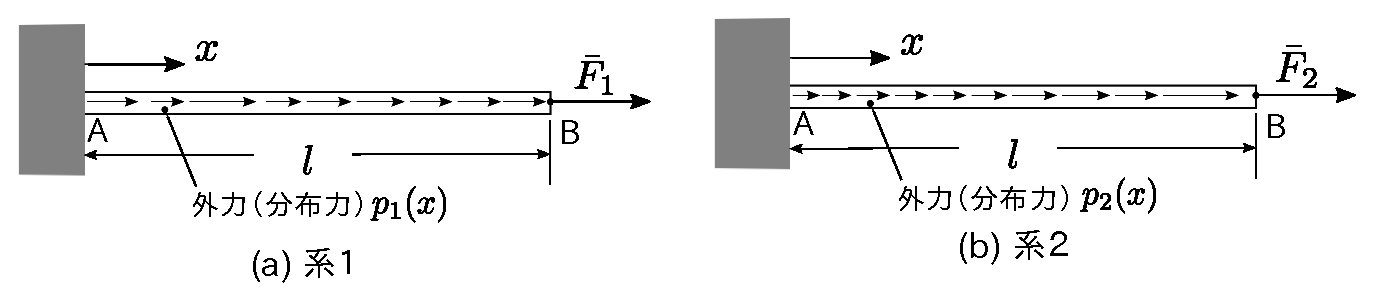
\includegraphics[width=0.8\linewidth]{fig1_2.eps} 
	\end{center}
	\caption{外力のみが異なる2つの系1と2.} 
	\label{fig:fig1_2}
\end{figure}
ここで式(\ref{eqn:WF_N})において,$u=u_1$, $\xi=u_2$とすれば,
\begin{equation}
	a(u_1,u_2)=\int_0^l N_1u_2'dx = \int_0^l\frac{N_1N_2}{EA}dx
	\label{eqn:vw_int}
\end{equation}
\begin{equation}
	b(u_2)=\bar F_1 u_2(l)+\int_0^l p_1 u_2dx
	\label{eqn:vw_ext}
\end{equation}
となる.ここで,式(\ref{eqn:vw_int})と式(\ref{eqn:vw_ext})は,ともに
力$\times$長さ,すなわち仕事の次元を持つ量となっている.
前者は内力である$N_1$, 後者は外力$\bar F_1$と$p_1(x)$に関するものである
ことから,これらの量をそれぞれ,内部仮想仕事,外部仮想仕事と呼ぶ.
"仮想"と呼ぶ理由は,力は系1の,変位は系2に関するものであることから,
両者の積が物理的に存在する仕事を指す訳ではないことによる.
系1と系2の間に成り立つ関係
\begin{equation}
	a(u_1,u_2)=b(u_2)
	\label{eqn:vw_eq}
\end{equation}
を,仮想仕事式と呼ぶ.
\subsection{単位荷重法}
仮想仕事式(\ref{eqn:vw_eq})における系1として,次のような特別な場合を考える.
\begin{equation}
	\bar F_1=0, \ \ p_1(x)=\delta(x-a), \ \ (0<a<l)
	\label{eqn:sys1}
\end{equation}
すなわち,系1として$x=a$に単位集中荷重だけが作用する場合を考える.
このとき,デルタ関数の性質
\begin{equation}
	\int_{-\infty}^{+\infty} f(x) \delta(x)dx =f(0)
	\label{eqn:dlt_sampling}
\end{equation}
を用いれば,式(\ref{eqn:vw_ext})は次のようになる. 
ただし$f(x)$は実数軸上全体で定義された任意の関数である.
よって
\begin{equation}
	b(u_2)=\int_0^l \delta(x-a)u_2(x)dx= u_2(a)
	\label{eqn:vw_eq_dlt}
\end{equation}
とすることができ,これを仮想仕事式(\ref{eqn:vw_eq})に代入すれば,
\begin{equation}
	u_2(a)=\int_0^l \frac{N_1N_2}{EA}dx
	\label{eqn:u2_a}
\end{equation}
の結果を得る.これは,2つの系1と2における軸力$N_1, N_2$から,系2の$x=a$
における変位$u_2(a)$を求めることができることを意味する.
言い換えれば,系1を変位計算の補助に用いることで,系2の変位を微分方程式を
直接解くこと無く得ることができることを意味している.
そこで, 系1を補助系,系2を解くべき問題とみる立場がより明確になるように,
2つの系に関する諸量を,あらためて 
\begin{eqnarray}
	\left( u_1, N_1; \bar F_1, p_1 \right)& = &
		\left(\tilde u, \tilde N;\, \bar{\tilde{F}}=0, \tilde p= \delta(x-a) \right) 
	\label{eqn:aux}
	\\
	\left( u_2, N_2; \bar F_2, p_2 \right)& = &
		\left( u,  N;\, \bar F, p \right) 
	\label{eqn:prb}
\end{eqnarray}
と書き直す.このとき式(\ref{eqn:u2_a})は,
\begin{equation}
	u(a)=\int_0^l \frac{N \tilde N}{EA}dx
	\label{eqn:uload}
\end{equation}
と表される.式(\ref{eqn:uload})を利用して変位の計算を行う解法を単位荷重法と呼ぶ.
\begin{figure}[h]
	\begin{center}
	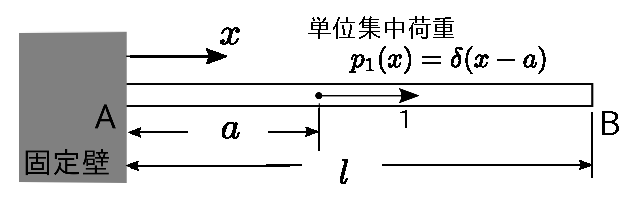
\includegraphics[width=0.4\linewidth]{fig1_3.eps} 
	\end{center}
	\caption{$x=a$に部材軸方向への単位集中荷重を受ける棒部材.} 
	\label{fig:fig1_3}
\end{figure}
%
\subsubsection{例題}
図\ref{fig:fig1_4}-(a)に示す棒部材の点Bと点Cに発生する軸変位を,単位荷重法を用いて求めよ.
断面剛性$EA$は全断面で一定とする.
\begin{figure}[h]
	\begin{center}
	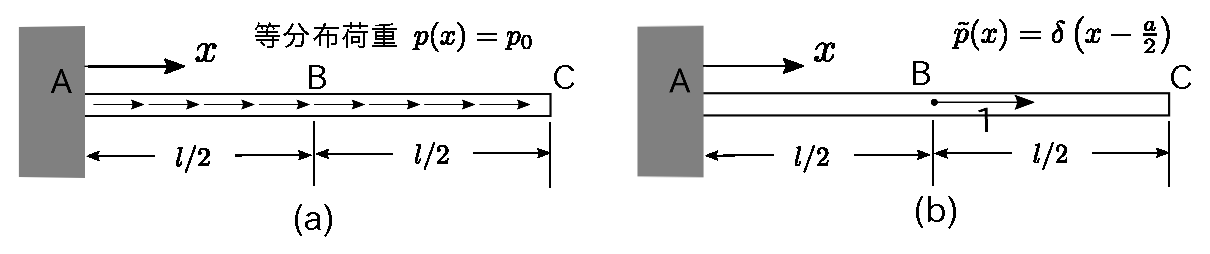
\includegraphics[width=0.8\linewidth]{fig1_4.eps} 
	\end{center}
	\caption{(a)等分布荷重を受ける棒部材(問題). (b)単位荷重法の適用において用いる補助系.} 
	\label{fig:fig1_4}
\end{figure}
\subsubsection{問題}
図\ref{fig:fig1_5}に示す3種類の系について,以下の問に答えよ.
なお,断面剛性$EA$は全ての部材,全ての断面で一定とする.
\begin{enumerate}
\item
	図\ref{fig:fig1_5}-(a)に示す棒部材の, 点Cにおける軸変位を求めよ.
\item
	図\ref{fig:fig1_5}-(a)に示す棒部材の, 点Bにおける軸変位を求めよ.
\item
	図\ref{fig:fig1_5}-(b)に示す棒部材に作用する支点反力を求め, 点Bにおける軸変位を求めよ.
\item
	図\ref{fig:fig1_5}-(c)に示す棒部材に作用する支点反力を求め, 点Bにおける軸変位を求めよ.
\end{enumerate}
\begin{figure}[h]
	\begin{center}
	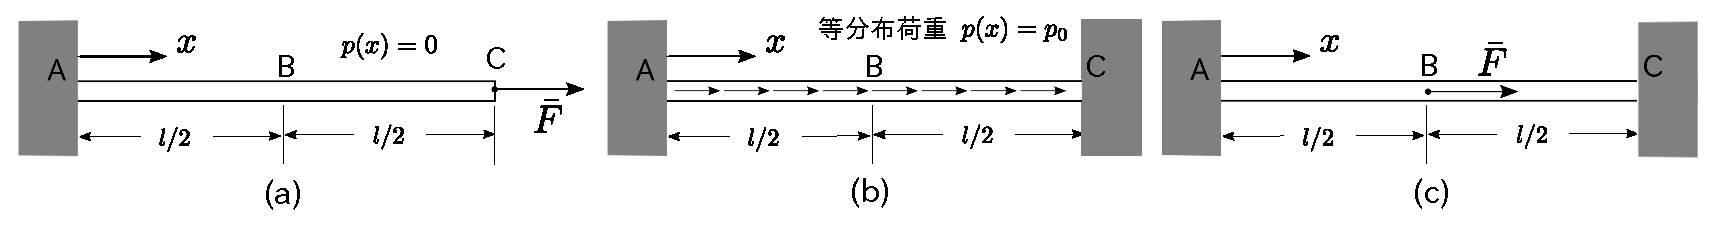
\includegraphics[width=1.0\linewidth]{fig1_5.eps} 
	\end{center}
	\caption{支持条件と荷重条件の異なる3種類の系.} 
	\label{fig:fig1_5}
\end{figure}
\end{document}

\subsection{変形に関する諸量}
断面位置を表すための座標を$x$,区間$a<x<b$における伸びを$\Delta l (a,b)$
と書く.このとき,区間$(a,b)$における平均ひずみ$\overline{\varepsilon}(a,b)$
を次式で定義する.
\begin{equation}
	\overline{\varepsilon}(a,b) =\frac{\Delta l (a,b)}{b-a}
	\label{eqn:eps_bar}
\end{equation}
このとき,$b \rightarrow a$の極限:
\begin{equation}
	\varepsilon(a)=\lim_{b \rightarrow a}\overline{\varepsilon}(a,b)
	\label{eqn:eps_def}
\end{equation}
を, 位置$x=a$のひずみと呼び, $x=a$における変形を表す量として用いる. 
$\varepsilon(a)$は, $x$における変位を$u(x)$と表すとき,
\begin{equation}
	\Delta l(a,b)=u(b)-u(a)
	\label{eqn:dell_u}
\end{equation}
であることから, $u$と$\varepsilon$の間には
\begin{equation}
	\varepsilon(a) = \lim _{b\rightarrow a} \frac{u(b)-u(a)}{b-a}= \left.\frac{du}{dx}\right|_{x=a}
	\label{eqn:eps_u}
\end{equation}
の関係がある.従って, ひずみと変位の関係は
\begin{equation}
	\varepsilon=\frac{du}{dx}
	\label{eqn:e_dudx}
\end{equation}
あるいは
\begin{equation}
	u(b)-u(a)=\int_{x'=a}^{x'=b} \varepsilon(x') dx'
	\label{eqn:u_int_eps}
\end{equation}
と表される.もし, $u(a)=0$となるように$a$を選ぶことができるならば, 
$b=x$と置き換え, $a$をそのように選ぶことで 式(\ref{eqn:u_int_eps})を
\begin{equation}
	u(x)=\int_{x'=a}^{x'=x} \varepsilon(x') dx'
	\label{eqn:u_int_eps0}
\end{equation}
とすることができる.
\paragraph{問題}
\begin{enumerate}
\item
長さ$l$の棒部材に,図\ref{fig:fig1}に示すような変位が発生しているとする.
このとき, ひずみ$\varepsilon(x)$を求め, その結果をグラフとして示せ.
ただし, 図中の$x$は棒部材の軸方向に沿って取った座標を表し, その原点$x=0$
は棒部材の一方の端部に位置するものとする.
\item
図\ref{fig:fig2}のように, 一端が固定された長さ$l$の棒部材に,
同図(a)〜(c)に示すひずみが発生しているとする.このとき, 変位$u(x)$を求め, 
その結果をグラフとして示すとともに, 区間$(0,l)$, $(0,l/2)$および$(l/2,l)$に
おける伸びを, (a)から(c)それぞれのひずみ分布に対して求めよ.
\end{enumerate}
\begin{figure}[h]
	\begin{center}
	\includegraphics[width=0.9\linewidth]{ex1_disp.eps} 
	\end{center}
	\caption{棒部材中の変位分布を表すグラフ.} 
	\label{fig:fig1}
\end{figure}
\begin{figure}[h]
	\begin{center}
	\includegraphics[width=0.9\linewidth]{ex2_strain.eps} 
	\end{center}
	\caption{棒部材中のひずみ分布を表すグラフ.} 
	\label{fig:fig2}
\end{figure}
%%%%%%%%%%%%%%%%%%%%%%%%%%%%%%%%%%%%%%%%%%%%%%%%%%%%%%%%
\newpage
\subsection{力に関する諸量}
棒部材の長手方向に働く, 単位長さあたりの外力を$p(x)$と表し, これを分布力
(正確には分布外力)あるいは物体力と呼ぶ. 区間$(a,b)$に作用する分布力の合力を
$P(a,b)$と表すとき, $P(a,b)$は
\begin{equation}
	P(a,b)=\int_{x'=a}^{x'=b}p(x')dx'=P(b)-P(a)
	\label{eqn:Pab}
\end{equation}
で得られる.ただし, 式(\ref{eqn:Pab})最右辺の$P(x)$は, $p(x)$の
任意の原始関数を表す.

位置$x$における軸力を$N(x)$, 断面積を$A(x)$とする.
軸力は外力に対する応答として部材内に発生する内力の一種である.
外力と内力は, 部材が静止状態にあるとき, 任意の区間で釣り合っている
必要がある. よって, 
任意の$0<a<b<l$に対して
\begin{equation}
	P(a,b)+N(b)-N(a)=0
	\label{eqn:Pab_equib}
\end{equation}
が成り立つ.式(\ref{eqn:Pab_equib})において$a=x, b=x+\Delta x$として, 
両辺を$\Delta x$で割り, その後$\Delta x\rightarrow 0$の極限をとれば
\begin{equation}
	\frac{P(x+\Delta x)-P(x)}{\Delta x}+\frac{N(x+\Delta x)-N(x)}{\Delta x}=0 \,\,
	\rightarrow
	\, \,
	\frac{dP}{dx}+\frac{dN}{dx}=0
	\label{eqn:Pab_equib_lim}
\end{equation}
となる. さらに,$P'(x)=p(x)$を用いれば式(\ref{eqn:Pab_equib_lim})より
\begin{equation}
	\frac{dN}{dx}+p=0
	\label{eqn:Nx_equib}
\end{equation}
が得られ, これも軸力の釣り合い式を表す. 
1次元軸力問題では部材断面に垂直に働く単位面積あたりの力:
\begin{equation}
	\sigma(x) = \frac{N(x)}{A(x)}
	\label{eqn:sigma1D_def}
\end{equation}
を応力と呼ぶ. 従って, 応力の釣り合い方程式は式(\ref{eqn:sigma1D_def})と
式(\ref{eqn:Nx_equib})より
\begin{equation}
	\frac{d\sigma A}{dx}+p=0
	\label{eqn:sigx_equib}
\end{equation}
となる.
\paragraph{力の単位}
科学,工学の分野では通常MKS単位系で各種の量が表される.すなわち, 
長さはメートル[m], 質量はキログラム[kg], 時間は秒[s]が単位として用いられる.
力は,ニュートンの第二法則によれば,質量×加速度の次元を持つことから, 
その単位は[kg$\cdot$m/s$^2$]であり,これをニュートン[N]と呼ぶ.
これに対して日常生活では,キログラム重[kgf]が力の単位としてしばしば
用いられる.キログラム重は, 質量1[kg]の物体が地球上で受ける重力の
大きさとして定義される.従って,Nとkgの換算は
\begin{center}
	1[kgf]=1[kg] $\times$ (重力加速度  $g\simeq$=9.8[m/s$^2$])=9.8[N]
\end{center}
で行うことができる.一方,応力や圧力の次元は,単位面積あたりの力である.よって
その単位は[N/m$^2$]であり,これをパスカル[Pa]と呼ぶ.
問題となる数量が非常に大きい,あるいは小さいとき,
その数値を適当な接頭辞を用いて表すことが多い.例えば,
10$^6$[Pa]は1[MPa](メガパスカル), 10$^{-6}$[s]は1[$\mu$s](マイクロ秒)等と
書くことができる.
\paragraph{問題}
図\ref{fig:fig3}に示すような, 左端が固定された, 長さ$l$の棒部材に, 
外力が作用している.このとき, 部材内部に発生する軸力$N$の分布を求め, 
その結果をグラフとして示せ.また, 棒部材が固定壁から受ける力(反力)を
(a)から(c)それぞれの場合について求めよ.
\begin{figure}[h]
	\begin{center}
	\includegraphics[width=0.9\linewidth]{ex3_force.eps} 
	\end{center}
	\caption{軸方向の外力を受ける棒部材.(a),(b)は集中荷重を,(c)は分布荷重を受ける
	部材を表す.(c)-iからiiiは,部材各点における分布荷重の大きさを表すグラフ.} 
	\label{fig:fig3}
\end{figure}
\subsection{境界値問題としての軸力問題}
応力$\sigma$とひずみ$\varepsilon$が, 比例係数$E$を用いて
\begin{equation}
	\sigma(x) =E(x) \varepsilon (x)
	\label{eqn:Hooke}
\end{equation}
と表されるような物体はフック固体と呼ばれ, 式(\ref{eqn:Hooke})の関係は
フック則を表す. 式(\ref{eqn:Hooke})を応力の釣り合い式(\ref{eqn:sigx_equib})に代入し, 
ひずみと変位の関係(\ref{eqn:e_dudx})を用いれば, 
変位に関する次の2階常微分方程式:
\begin{equation}
	\frac{d}{dx}\left( EA \frac{du}{dx} \right)+p=0
	\label{eqn:gvn_eq}
\end{equation}
が得られる. この微分方程式を適切な境界条件(支持条件)の元で解けば, 
変位分布が求められ, その結果を微分することでひずみ$\varepsilon$や
応力$\sigma$, 軸力$N$が得られる.

棒部材の支持条件(境界条件)には種々のものが考えられるが,以下のタイプが最も基本的である。
\begin{itemize}
\item
変位境界(固定端を含む): $u(b)=\bar{u}$\\
	($x=b$は境界位置の座標を, $\bar u$は与えられた変位量を表す。
	$\bar u=0$は固定端に相当する)
\item
荷重境界(自由端を含む):$N(b)=\bar{N}$\\
	 ($x=b$は境界位置の座標を, $\bar N$は与えられた外力を表す.
	$\bar{N}$は, 引張を正とする. $\bar N=0$は自由端に相当する)
\end{itemize}
断面剛性$EA$が場所によらず一定のとき,式(\ref{eqn:gvn_eq})は
\begin{equation}
	EA\frac{d^2u}{dx^2}+p=0
	\label{eqn:gvn_eq2}
\end{equation}
と,定数係数の2階線形常微分方程式となる.
\paragraph{問題}
図\ref{fig:fig4}に示す(a)から(c)のような棒部材について, 
変位と軸力分布を求め, その結果をグラフとして示せ.また, 各々の場合について, 
支点反力を求めよ.ただし, 図中に示した$p(x)$は分布力を意味し,断面剛性
$EA$は場所によらず一定とする.
\begin{figure}[h]
	\begin{center}
	\includegraphics[width=0.9\linewidth]{ex4_ODE.eps} 
	\end{center}
	\caption{軸方向の外力を受ける棒部材.$p=p(x)$は分布力を,$p_0$は与えられた定数を意味し, 
	断面剛性$EA$は場所によらず一定とする.} 
	\label{fig:fig4}
\end{figure}
%%%%%%%%%%%%%%%%%
%%%%%%%%%%%%%%%%%
\clearpage
\subsection{補足}
%\subsubsection{接頭辞}
\begin{table}[h]
\begin{center}
\caption{よく利用される数値に関する接頭辞(metric prefix)}
\label{tbl:prefix}
\begin{tabular}{c|c|c|c|c|c|c|c|c|c|c}
f & p & n & $\mu$ & m & & k & M & G & T & P \\
\hline
フェムト & ピコ& ナノ & マイクロ & ミリ & & キロ & メガ& ギガ& テラ & ペタ\\
\hline
$10^{-15}$ &
$10^{-12}$&
$10^{-9}$ &
$10^{-6}$ &
$10^{-3}$ &
$10^0$ &
$10^3$ &
$10^6$ &
$10^9$ &
$10^{12}$&
$10^{15}$ 
\end{tabular}
\end{center}
\end{table}
%\subsubsection{ギリシャ文字}
\begin{table}[h]
\begin{center}
\caption{ギリシャ文字とその読み方}
\begin{tabular}{c|c|c|c}
大文字 & 小文字 & 読み方(英語) &読み方(日本語)\\
\hline \hline
$A$ & $\alpha$ & alpha & アルファ \\
\hline
$B$ & $\beta$ & beta & ベータ \\
\hline
$\Gamma$ & $\gamma$ & gamma & ガンマ\\
\hline
$\Delta$ & $\delta$ & delta & デルタ\\
\hline
$E$ & $\epsilon, \varepsilon$ & epsilon & イプシロン \\
\hline
$Z$ & $\zeta$ & zeta & ゼータ \\
\hline
$H$ & $\eta$ & eta & イータ \\
\hline
$\Theta$ & $\theta$ & theta & シータ \\
\hline
$I$ & $\iota$ & iota & イオタ \\
\hline
$K$ & $\kappa$ & kappa & カッパ\\
\hline
$\Lambda$ & $\lambda$ & lambda & ラムダ \\
\hline
$M$ & $\mu$ & mu & ミュー \\
\hline
$N$ & $\nu$ & nu & ニュー\\
\hline
$\Xi$ & $\xi$ & xi & グザイ\\
\hline
$O$ & $o$ & omicron & オミクロン\\
\hline
$\Pi$ & $\pi,\varpi$ & pi & パイ \\
\hline
$P$ & $\rho$ & rho & ロー \\
\hline
$\Sigma$ & $\sigma$ & sigma & シグマ\\
\hline
$T$ & $\tau$ & tau &タウ \\
\hline
$\Upsilon$ & $\upsilon$ & upsilon & ウプシロン\\
\hline
$\Phi$ & $\phi, \varphi$ & phi &ファイ \\
\hline
$X$ & $\chi$ & chi & カイ \\
\hline
$\Psi$ & $\psi$ & psi & プサイ \\
\hline
$\Omega$ & $\omega$ & omega & オメガ\\
\end{tabular}
\end{center}
\end{table}
%%%%%%%%%%%%%%%%%%%%%%%%
\end{document}
%\begin{figure}[here]
\begin{figure}
	\vspace{-3mm}
	\begin{center}
	\includegraphics[width=0.45\linewidth]{fig1.eps} 
	\end{center}
	\vspace{-5mm}
	\caption{一端を固定壁に支持された棒部材とそのひずみ分布.} 
	\label{fig:fig1}
\end{figure}
%%%%%%%%%%%%%%%%%%%%%%%%%%%%%%%%%%%%%%%%%%%%

